\documentclass[]{book}
\usepackage{lmodern}
\usepackage{amssymb,amsmath}
\usepackage{ifxetex,ifluatex}
\usepackage{fixltx2e} % provides \textsubscript
\ifnum 0\ifxetex 1\fi\ifluatex 1\fi=0 % if pdftex
  \usepackage[T1]{fontenc}
  \usepackage[utf8]{inputenc}
\else % if luatex or xelatex
  \ifxetex
    \usepackage{mathspec}
  \else
    \usepackage{fontspec}
  \fi
  \defaultfontfeatures{Ligatures=TeX,Scale=MatchLowercase}
\fi
% use upquote if available, for straight quotes in verbatim environments
\IfFileExists{upquote.sty}{\usepackage{upquote}}{}
% use microtype if available
\IfFileExists{microtype.sty}{%
\usepackage{microtype}
\UseMicrotypeSet[protrusion]{basicmath} % disable protrusion for tt fonts
}{}
\usepackage[margin=1in]{geometry}
\usepackage{hyperref}
\hypersetup{unicode=true,
            pdftitle={Estadística descriptiva},
            pdfauthor={Ángel Berihuete, Carmen Ramos, Juan Antonio García},
            pdfborder={0 0 0},
            breaklinks=true}
\urlstyle{same}  % don't use monospace font for urls
\usepackage{natbib}
\bibliographystyle{apalike}
\usepackage{color}
\usepackage{fancyvrb}
\newcommand{\VerbBar}{|}
\newcommand{\VERB}{\Verb[commandchars=\\\{\}]}
\DefineVerbatimEnvironment{Highlighting}{Verbatim}{commandchars=\\\{\}}
% Add ',fontsize=\small' for more characters per line
\usepackage{framed}
\definecolor{shadecolor}{RGB}{248,248,248}
\newenvironment{Shaded}{\begin{snugshade}}{\end{snugshade}}
\newcommand{\KeywordTok}[1]{\textcolor[rgb]{0.13,0.29,0.53}{\textbf{#1}}}
\newcommand{\DataTypeTok}[1]{\textcolor[rgb]{0.13,0.29,0.53}{#1}}
\newcommand{\DecValTok}[1]{\textcolor[rgb]{0.00,0.00,0.81}{#1}}
\newcommand{\BaseNTok}[1]{\textcolor[rgb]{0.00,0.00,0.81}{#1}}
\newcommand{\FloatTok}[1]{\textcolor[rgb]{0.00,0.00,0.81}{#1}}
\newcommand{\ConstantTok}[1]{\textcolor[rgb]{0.00,0.00,0.00}{#1}}
\newcommand{\CharTok}[1]{\textcolor[rgb]{0.31,0.60,0.02}{#1}}
\newcommand{\SpecialCharTok}[1]{\textcolor[rgb]{0.00,0.00,0.00}{#1}}
\newcommand{\StringTok}[1]{\textcolor[rgb]{0.31,0.60,0.02}{#1}}
\newcommand{\VerbatimStringTok}[1]{\textcolor[rgb]{0.31,0.60,0.02}{#1}}
\newcommand{\SpecialStringTok}[1]{\textcolor[rgb]{0.31,0.60,0.02}{#1}}
\newcommand{\ImportTok}[1]{#1}
\newcommand{\CommentTok}[1]{\textcolor[rgb]{0.56,0.35,0.01}{\textit{#1}}}
\newcommand{\DocumentationTok}[1]{\textcolor[rgb]{0.56,0.35,0.01}{\textbf{\textit{#1}}}}
\newcommand{\AnnotationTok}[1]{\textcolor[rgb]{0.56,0.35,0.01}{\textbf{\textit{#1}}}}
\newcommand{\CommentVarTok}[1]{\textcolor[rgb]{0.56,0.35,0.01}{\textbf{\textit{#1}}}}
\newcommand{\OtherTok}[1]{\textcolor[rgb]{0.56,0.35,0.01}{#1}}
\newcommand{\FunctionTok}[1]{\textcolor[rgb]{0.00,0.00,0.00}{#1}}
\newcommand{\VariableTok}[1]{\textcolor[rgb]{0.00,0.00,0.00}{#1}}
\newcommand{\ControlFlowTok}[1]{\textcolor[rgb]{0.13,0.29,0.53}{\textbf{#1}}}
\newcommand{\OperatorTok}[1]{\textcolor[rgb]{0.81,0.36,0.00}{\textbf{#1}}}
\newcommand{\BuiltInTok}[1]{#1}
\newcommand{\ExtensionTok}[1]{#1}
\newcommand{\PreprocessorTok}[1]{\textcolor[rgb]{0.56,0.35,0.01}{\textit{#1}}}
\newcommand{\AttributeTok}[1]{\textcolor[rgb]{0.77,0.63,0.00}{#1}}
\newcommand{\RegionMarkerTok}[1]{#1}
\newcommand{\InformationTok}[1]{\textcolor[rgb]{0.56,0.35,0.01}{\textbf{\textit{#1}}}}
\newcommand{\WarningTok}[1]{\textcolor[rgb]{0.56,0.35,0.01}{\textbf{\textit{#1}}}}
\newcommand{\AlertTok}[1]{\textcolor[rgb]{0.94,0.16,0.16}{#1}}
\newcommand{\ErrorTok}[1]{\textcolor[rgb]{0.64,0.00,0.00}{\textbf{#1}}}
\newcommand{\NormalTok}[1]{#1}
\usepackage{longtable,booktabs}
\usepackage{graphicx,grffile}
\makeatletter
\def\maxwidth{\ifdim\Gin@nat@width>\linewidth\linewidth\else\Gin@nat@width\fi}
\def\maxheight{\ifdim\Gin@nat@height>\textheight\textheight\else\Gin@nat@height\fi}
\makeatother
% Scale images if necessary, so that they will not overflow the page
% margins by default, and it is still possible to overwrite the defaults
% using explicit options in \includegraphics[width, height, ...]{}
\setkeys{Gin}{width=\maxwidth,height=\maxheight,keepaspectratio}
\IfFileExists{parskip.sty}{%
\usepackage{parskip}
}{% else
\setlength{\parindent}{0pt}
\setlength{\parskip}{6pt plus 2pt minus 1pt}
}
\setlength{\emergencystretch}{3em}  % prevent overfull lines
\providecommand{\tightlist}{%
  \setlength{\itemsep}{0pt}\setlength{\parskip}{0pt}}
\setcounter{secnumdepth}{5}
% Redefines (sub)paragraphs to behave more like sections
\ifx\paragraph\undefined\else
\let\oldparagraph\paragraph
\renewcommand{\paragraph}[1]{\oldparagraph{#1}\mbox{}}
\fi
\ifx\subparagraph\undefined\else
\let\oldsubparagraph\subparagraph
\renewcommand{\subparagraph}[1]{\oldsubparagraph{#1}\mbox{}}
\fi

%%% Use protect on footnotes to avoid problems with footnotes in titles
\let\rmarkdownfootnote\footnote%
\def\footnote{\protect\rmarkdownfootnote}

%%% Change title format to be more compact
\usepackage{titling}

% Create subtitle command for use in maketitle
\newcommand{\subtitle}[1]{
  \posttitle{
    \begin{center}\large#1\end{center}
    }
}

\setlength{\droptitle}{-2em}

  \title{Estadística descriptiva}
    \pretitle{\vspace{\droptitle}\centering\huge}
  \posttitle{\par}
    \author{Ángel Berihuete, Carmen Ramos, Juan Antonio García}
    \preauthor{\centering\large\emph}
  \postauthor{\par}
      \predate{\centering\large\emph}
  \postdate{\par}
    \date{2018-11-14}

\usepackage{booktabs}
\ifxetex
  \usepackage{polyglossia}
  \setmainlanguage{spanish}
  % Tabla en lugar de cuadro
  \gappto\captionsspanish{\renewcommand{\tablename}{Tabla}  
          \renewcommand{\listtablename}{Índice de tablas}}
\else
  \usepackage[spanish,es-tabla]{babel}
\fi

\usepackage{amsthm}
\newtheorem{theorem}{Teorema}[chapter]
\newtheorem{lemma}{Lema}[chapter]
\newtheorem{corollary}{Corolario}[chapter]
\newtheorem{proposition}{Proposición}[chapter]
\newtheorem{conjecture}{Conjecture}[chapter]
\theoremstyle{definition}
\newtheorem{definition}{Definición}[chapter]
\theoremstyle{definition}
\newtheorem{example}{Ejemplo}[chapter]
\theoremstyle{definition}
\newtheorem{exercise}{Ejercicio}[chapter]
\theoremstyle{remark}
\newtheorem*{remark}{Nota: }
\newtheorem*{solution}{Solución}
\let\BeginKnitrBlock\begin \let\EndKnitrBlock\end
\begin{document}
\maketitle

{
\setcounter{tocdepth}{1}
\tableofcontents
}
\chapter*{Prólogo}\label{prologo}
\addcontentsline{toc}{chapter}{Prólogo}

Este libro es una recopilación de apuntes y presentaciones impartidos en
las clases de Estadística descriptiva. No es un libro completo. Al
contrario, se está insertando y actualizando material de manera
continua. ¡Cualquier sugerencia a través del repo en GitHub será
bienvenida!

El libro ha sido escrito en
\href{http://rmarkdown.rstudio.com}{R-Markdown} utilizando el paquete
\href{https://bookdown.org/yihui/bookdown/}{\texttt{bookdown}} y está
disponible en el repositorio Github:
\href{https://github.com/AngelBerihuete/EstNavBook}{AngelBerihuete/EstNavBook}.

Esta obra está bajo una licencia de
\href{https://creativecommons.org/licenses/by-sa/4.0/deed.es}{Creative
Commons Reconocimiento-CompartirIgual 4.0 Internacional}.

\begin{flushleft}
\includegraphics[width=1.22in]{images/by-sa-88x31} \end{flushleft}

\chapter{Introducción al análisis de datos}\label{intro}

En las siguientes secciones iremos desarrollando los elementos básicos
de un análisis exploratorio, calculando medidas que nos ayuden a
interpretar de forma adecuada el conjunto de datos analizados. Para ello
utilizaremos varios conjuntos de datos que podrán ser descargados del
\href{https://github.com/AngelBerihuete/EstNavBook/tree/master/datasets}{repositorio}
en GitHub.

Planteamos el siguiente problema sencillo: los precios (en euros) de un
conjunto de botellas de vino en cierta sección de un centro comercial
son los siguientes

42 42 42 42 42 42 42 42 42 42 42 42 42 42 42 42 42 42 42 42 43 43 43 43
43 43 43 43 43 43 43 43 43 43 43 52 52 52 52 52 52 52 52 52 52 52 52 52
52 52 52 52 52 52 52 53 53 53 53 53 53 53 53 53 53 62 62 62 62 62 62 62
62 62 63 63 63 63 63

Podríamos hacernos las siguientes preguntas:

\begin{enumerate}
\def\labelenumi{\arabic{enumi}.}
\item
  ¿Cómo preparo los datos para su análisis?
\item
  ¿Qué representación gráfica hago de los datos?
\item
  ¿Puedo elegir uno o varios valores que representen con garantías al
  conjunto de los datos?
\item
  ¿Cómo puedo sistematizar el análisis de un conjunto de datos?
\end{enumerate}

Un \textbf{análisis exploratorio de datos} implica el uso de los
elementos numéricos y gráficos que describan lo más exhaustivamente
posible un conjunto de datos. Además, deberá poner de manifiesto los
aspectos más relevantes de la distribución de los datos: regularidades,
datos atípicos, especificidades, relaciones, etc.

En este capítulo nos marcamos los siguientes objetivos:

\begin{itemize}
\item
  Ser capaces de identificar el tipo de variable estadística en estudio.
\item
  Decidir qué tipo de medidas y gráficos serán los adecuados para
  resumir los diferentes tipos de variables estadísticas.
\item
  Entender que \textbf{la media no siempre es la adecuada para resumir
  los datos}.
\item
  Ser capaces de comparar diferentes medidas entre diferentes conjuntos
  de datos.
\item
  Diferenciar entre \textbf{análisis exploratorio} de datos e
  \textbf{inferencia estadística}.
\end{itemize}

\section{Variables estadísticas}\label{variables-estadisticas}

Las variables a analizar pueden ser de diferentes tipos:

\begin{itemize}
\item
  \textbf{Cualitativas} o \textbf{factores}: son variables no
  expresables numéricamente.
\item
  \textbf{Cuantitativas}: pueden ser expresadas numéricamente. Las
  variables cuantitativas se subdividen en:
\end{itemize}

\begin{enumerate}
\def\labelenumi{\arabic{enumi}.}
\item
  \textbf{Cuantitativas Discretas}, si el conjunto de sus posibles
  valores tiene cardinal finito o infinito numerable. (Ejemplo: ``Número
  de trabajadores en una bodega'')
\item
  \textbf{Cuantitativas Continuas}, si pueden tomar los infinitos
  valores de un intervalo.
\end{enumerate}

A veces, por cuestiones prácticas, conviene discretizar las variables
cuantitativas continuas. Por ejemplo la variable ``Antigüedad del vino
en una bota, medida en años''.

\section{Distribuciones de
frecuencias}\label{distribuciones-de-frecuencias}

A partir de un conjunto de datos queremos clasificarlos de modo que la
información contenida en ellos quede presentada de forma clara, concisa
y ordenada.

Si representamos por \(N\) al número total de datos, entre los que
consideraremos que hay \(k\) valores distintos \(x_1\),
\(x_2\),\ldots{}, \(x_k\) (que en el caso de las variables cuantitativas
se presentarán ordenados de menor a mayor), se conoce como
\textbf{frecuencia}:

\begin{itemize}
\item
  \textbf{Absoluta} del valor \(x_i\), al número de veces que se
  presenta dicho valor en el conjunto de datos. Se representa por
  \(n_i\).
\item
  \textbf{Absoluta acumulada} del valor \(x_i\), al número de datos que
  hay iguales o inferiores a \(x_i\). Se representa por \(N_i\).
\item
  \textbf{Relativa} del valor \(x_i\), al cociente \(\dfrac{n_i}{N}\).
  Se representa por \(f_i\).
\item
  \textbf{Relativa acumulada} del valor \(x_i\), al cociente
  \(\dfrac{N_i}{N}\). Se representa por \(F_i\).
\end{itemize}

\BeginKnitrBlock{example}[El problema del fluoruro]
\protect\hypertarget{exm:fluoruro}{}{\label{exm:fluoruro} \iffalse (El
problema del fluoruro) \fi{} }

Para realizar un estudio sobre el contenido en ion fluoruro en vinos
embotellados de mayor comercialización en Canarias se procedió al
análisis de 79 vinos embotellados de los cuales 50 son de la comunidad
de Canarias y 29 de la Península. La siguiente tabla muestra los 10
primeros registros:
\EndKnitrBlock{example}

denominacion

tipo

conc\_fluor

procedencia

precio

El Hierro

Tinto

0.13

Canarias

42

Ycoden Daute Isora

Tinto

0.07

Canarias

42

Ycoden Daute Isora

Tinto

0.10

Canarias

42

Ycoden Daute Isora

Tinto

0.11

Canarias

42

La Palma

Tinto

0.26

Canarias

42

Lanzarote

Tinto

0.12

Canarias

42

La tabla de frecuencias del factor tipo que tiene niveles Tinto, Blanco,
Rosado

\[ x_i \]

\[ n_i \]

\[ N_i \]

\[ f_i \]

\[ F_i \]

Blanco

27

27

0.3418

0.3418

Rosado

18

45

0.2278

0.5696

Tinto

34

79

0.4304

1.0000

siendo el gráfico más adecuado para esta variable el \textbf{diagrama de
sectores} o el \textbf{diagrama de barras}.

\begin{center}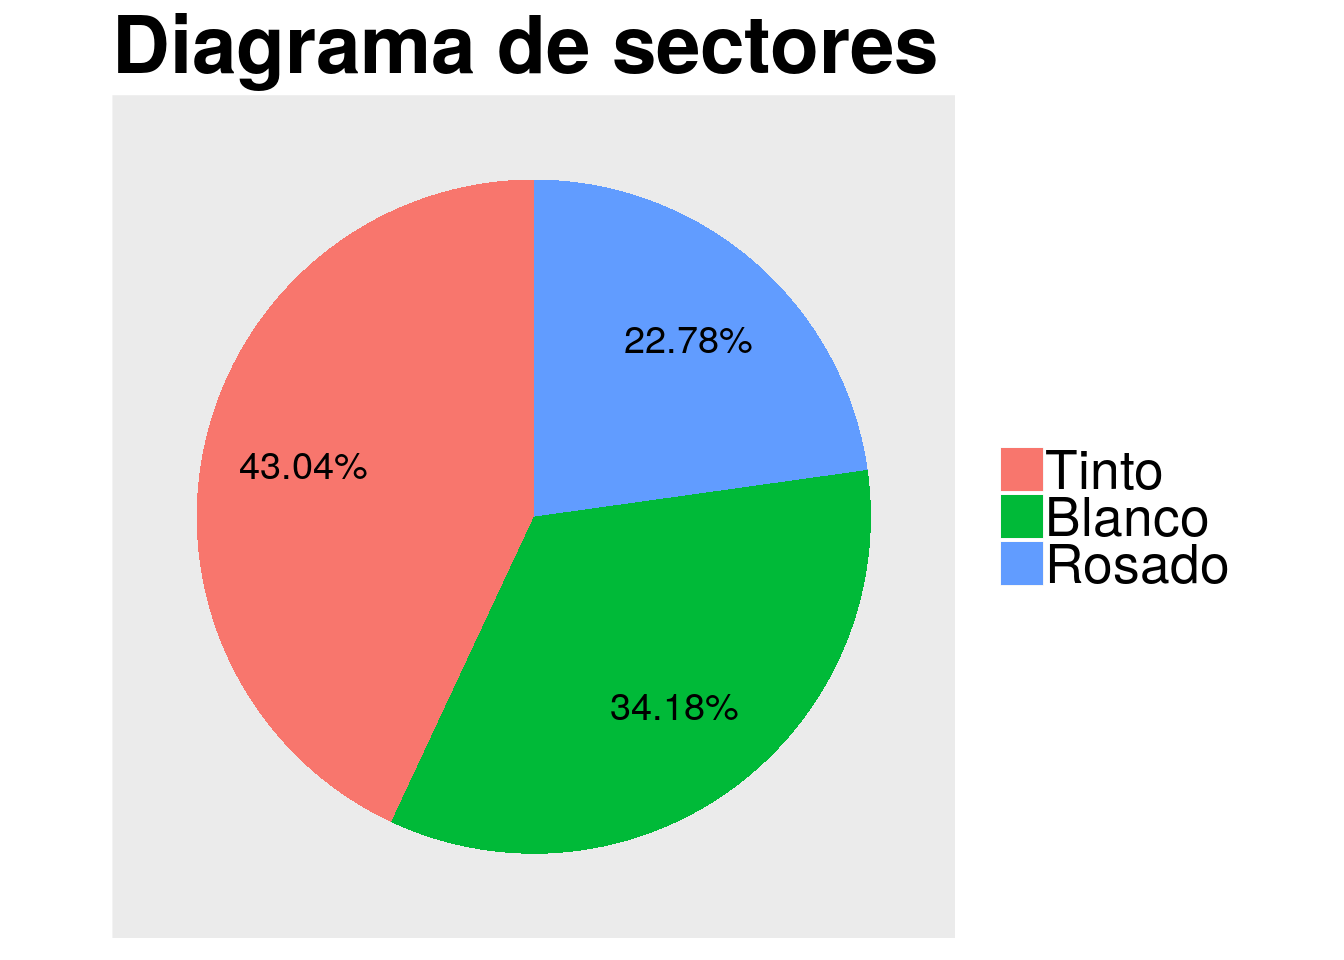
\includegraphics{01-AnalDatos_files/figure-latex/unnamed-chunk-4-1} \end{center}

\begin{center}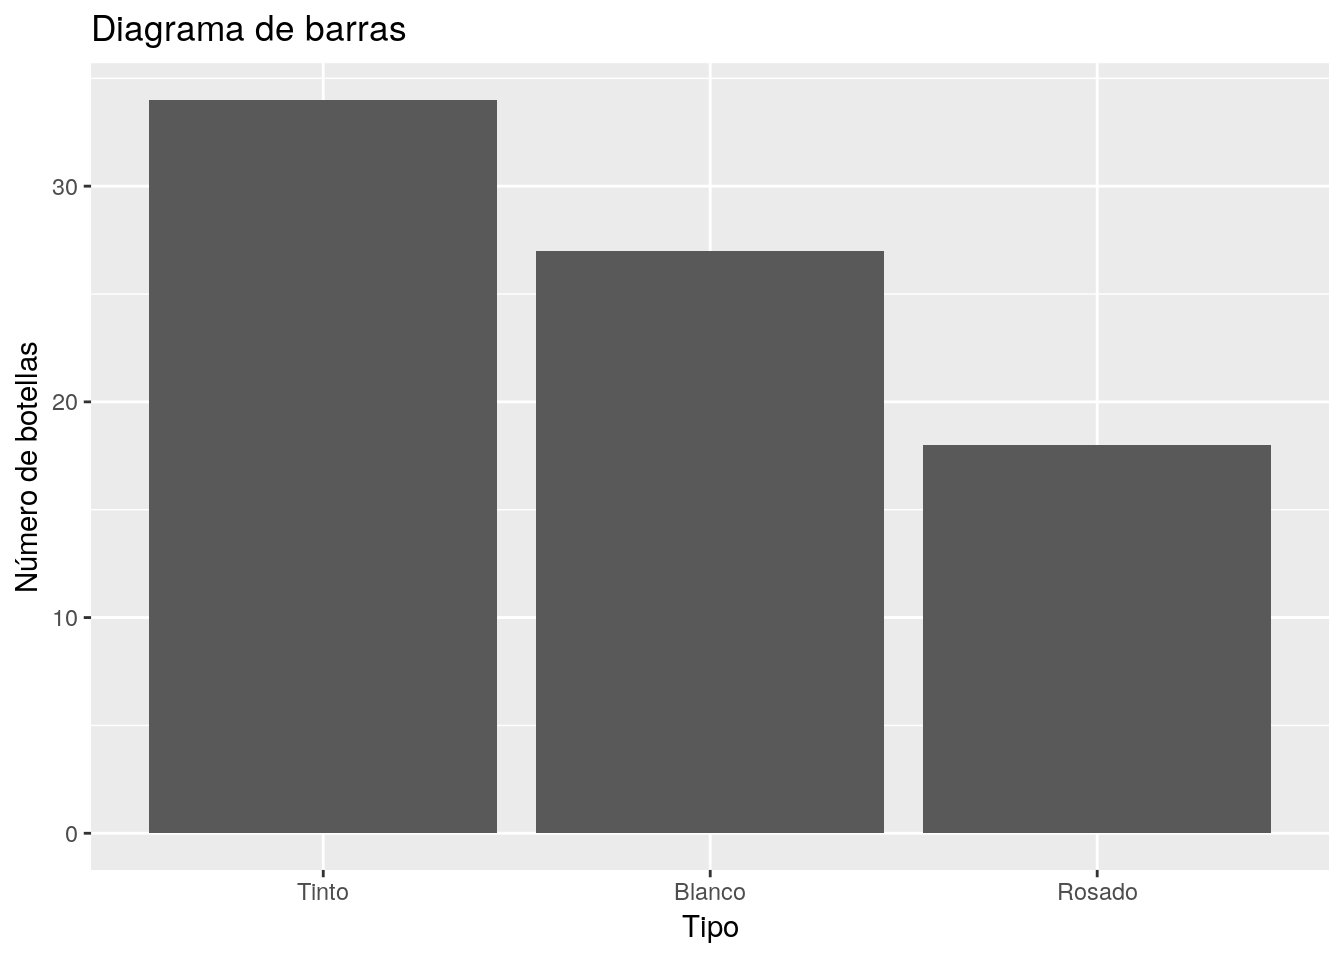
\includegraphics{01-AnalDatos_files/figure-latex/unnamed-chunk-5-1} \end{center}

\subsection{Variables cuantitativas
discretas}\label{variables-cuantitativas-discretas}

Tabla de frecuencias de la variable precio

42 42 42 42 42 42 42 42 42 42 42 42 42 42 42 42 42 42 42 42 43 43 43 43
43 43 43 43 43 43 43 43 43 43 43 52 52 52 52 52 52 52 52 52 52 52 52 52
52 52 52 52 52 52 52 53 53 53 53 53 53 53 53 53 53 62 62 62 62 62 62 62
62 62 63 63 63 63 63

\[ x_i \]

\[ n_i \]

\[ N_i \]

\[ f_i \]

\[ F_i \]

42

20

20

0.2532

0.2532

43

15

35

0.1899

0.4430

52

20

55

0.2532

0.6962

53

10

65

0.1266

0.8228

62

9

74

0.1139

0.9367

63

5

79

0.0633

1.0000

y el gráfico adecuado para este tipo de variable será el
\textbf{diagrama de barras}:

\begin{center}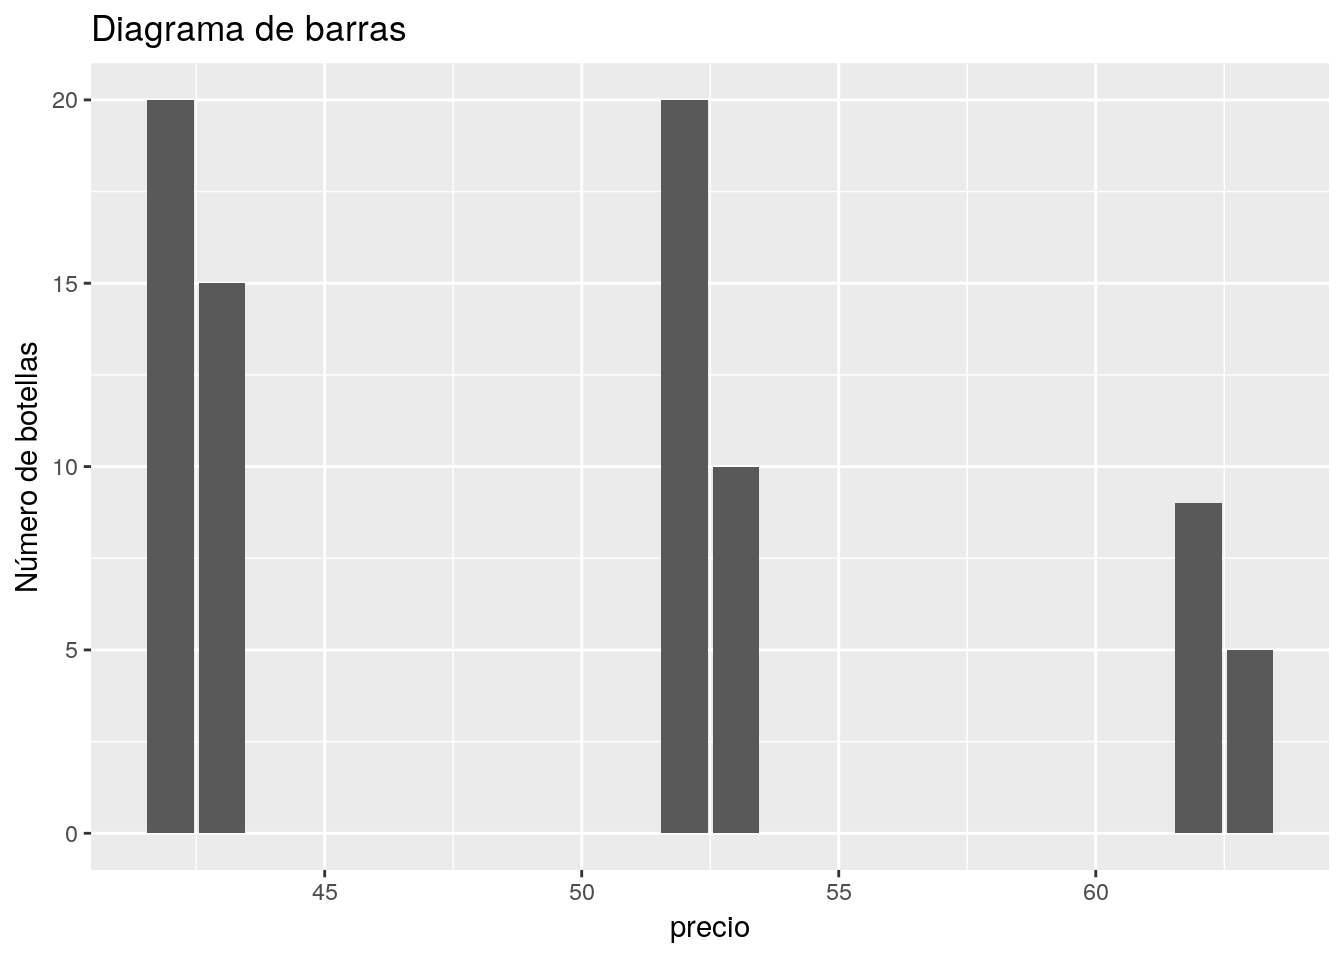
\includegraphics{01-AnalDatos_files/figure-latex/unnamed-chunk-7-1} \end{center}

\[ x_i \]

\[ n_i \]

\[ N_i \]

\[ f_i \]

\[ F_i \]

42

20

20

0.2532

0.2532

43

15

35

0.1899

0.4430

52

20

55

0.2532

0.6962

53

10

65

0.1266

0.8228

62

9

74

0.1139

0.9367

63

5

79

0.0633

1.0000

\subsection{Variables cuantitativas
continuas}\label{variables-cuantitativas-continuas}

La tabla de frecuencias de la variable cuantitativa continua conc\_fluor

\[ ( l_{i-1}, l_i ] \]

\[n_i\]

\[N_i\]

\[f_i\]

\[F_i\]

(0,0.2{]}

45

45

0.5696

0.5696

(0.2,0.3{]}

22

67

0.2785

0.8481

(0.3,0.4{]}

7

74

0.0886

0.9367

(0.4,0.6{]}

5

79

0.0633

1.0000

Obsérvese que hemos agrupado en intervalos los valores

0.13 0.07 0.10 0.11 0.26 0.12 0.20 0.17 0.08 0.14 0.17 0.13 0.16 0.16
0.15 0.28 0.18 0.20 0.09 0.13 0.13 0.06 0.13 0.22 0.12 0.14 0.12 0.17
0.12 0.50 0.15 0.22 0.13 0.20 0.18 0.13 0.10 0.10 0.18 0.09 0.15 0.15
0.08 0.11 0.16 0.17 0.10 0.09 0.15 0.18 0.25 0.26 0.27 0.28 0.28 0.29
0.27 0.27 0.28 0.44 0.37 0.46 0.24 0.28 0.33 0.37 0.46 0.22 0.28 0.38
0.29 0.27 0.29 0.29 0.36 0.23 0.32 0.36 0.45

El gráfico adecuado para este tipo de variable es el
\textbf{histograma}:

\begin{center}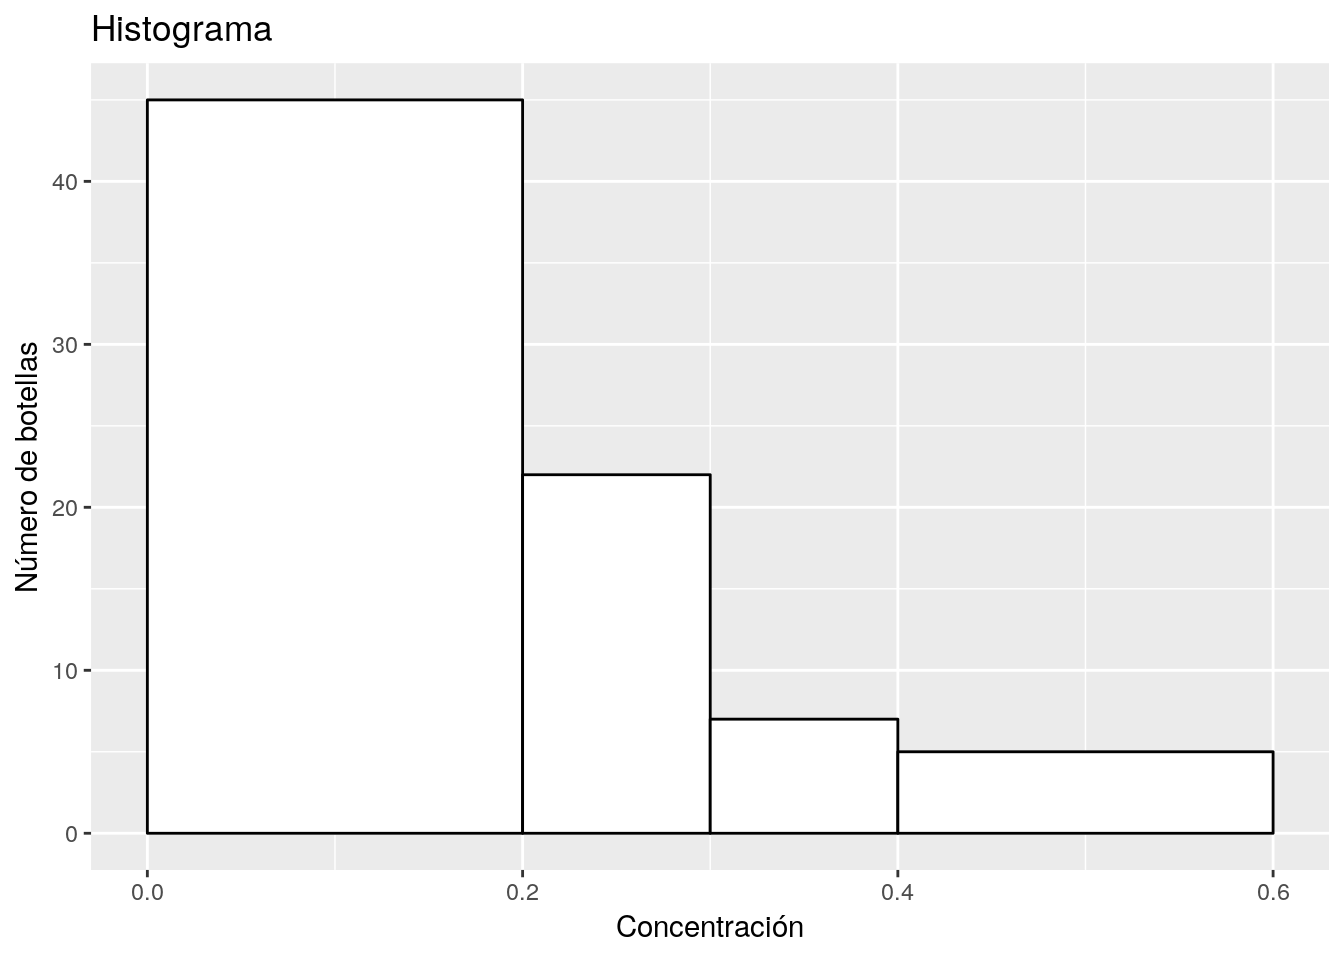
\includegraphics{01-AnalDatos_files/figure-latex/unnamed-chunk-10-1} \end{center}

¡Cuidado! Longitud de intervalos distinta. Tendremos que utilizar la
\textbf{densidad} \((h_i)\) para representar el histograma. Ahora la
tabla de frecuencias de la variable cuantitativa continua conc\_fluor

\[ ( l_{i-1}, l_i  ] \]

\[n_i\]

\[N_i\]

\[f_i\]

\[F_i\]

\[h_i\]

(0,0.2{]}

45

45

0.5696

0.5696

2.8481

(0.2,0.3{]}

22

67

0.2785

0.8481

2.7848

(0.3,0.4{]}

7

74

0.0886

0.9367

0.8861

(0.4,0.6{]}

5

79

0.0633

1.0000

0.3165

Siendo \(h_i = \frac{f_i}{a_i}\)

\begin{center}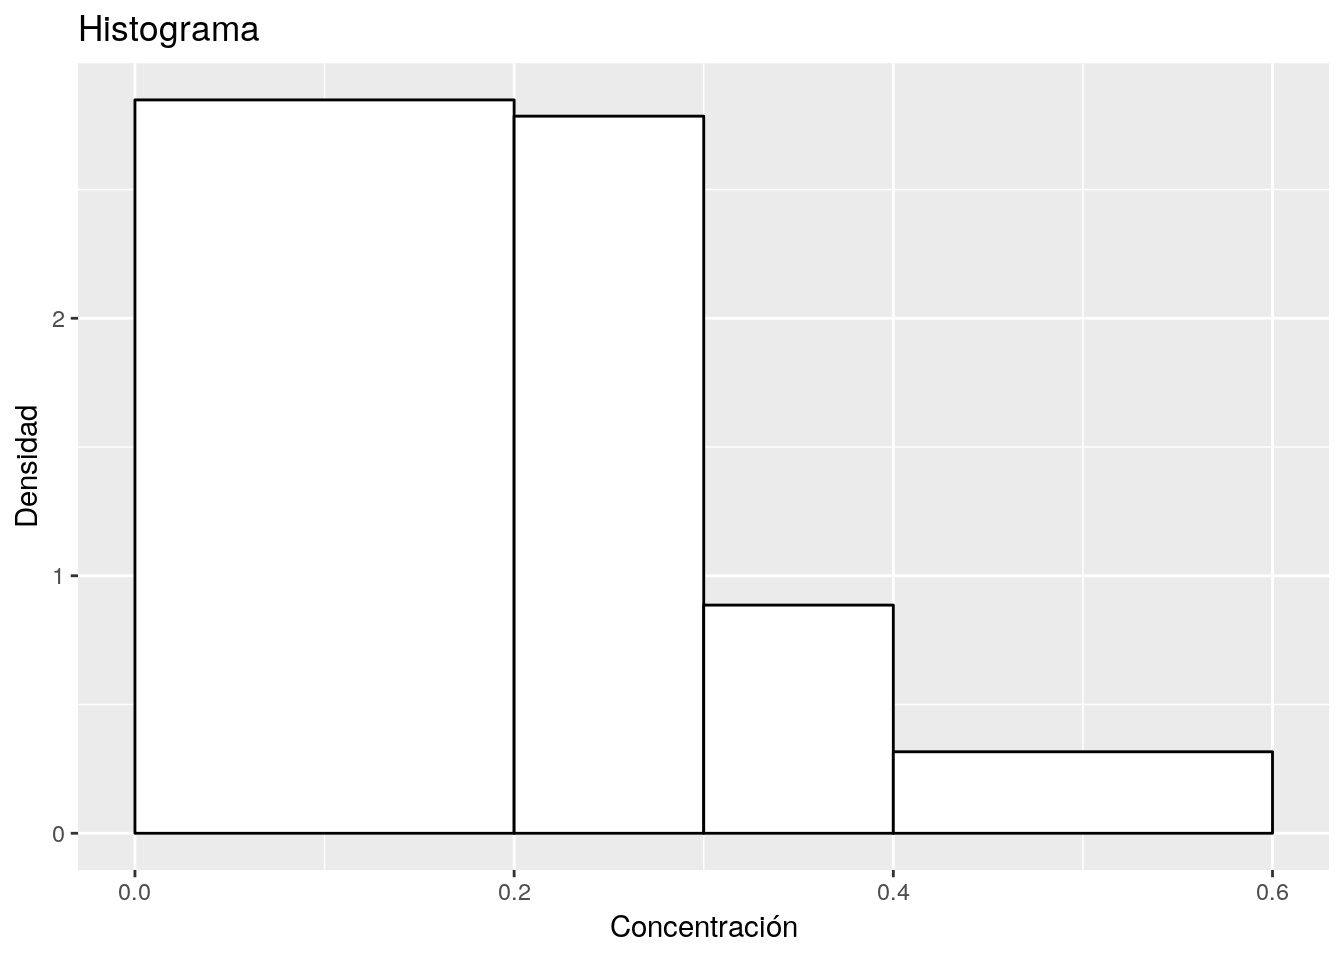
\includegraphics{01-AnalDatos_files/figure-latex/unnamed-chunk-12-1} \end{center}

\subsection{¿Qué número de intervalos y qué amplitud es la
adecuada?}\label{que-numero-de-intervalos-y-que-amplitud-es-la-adecuada}

No hay una fórmula con la que obtener un valor óptimo del número de
intervalos y su amplitud. Existen muchas dependiendo de las hipótesis
que hagamos en nuestro problema. Algunas de las más utilizadas si
tenemos \(N\) observaciones:

\begin{itemize}
\tightlist
\item
  \(k = \sqrt{N}\) lo usa de forma predefinida el programa Excel.
\item
  \(k = \lceil \log_2 N \rceil +1\) lo usa de forma predefinida el
  programa R. Da resultados pobres si \(n<30\) (Nota:
  \(\lceil 2.4 \rceil = 3\)).
\end{itemize}

Una vez tenemos el número de intervalos, basta calcular su amplitud
mediante

\[ a = \frac{\max{x} - \min{x}}{k} \]

\subsection{¿Pueden manipular nuestra opinión con los
gráficos?}\label{pueden-manipular-nuestra-opinion-con-los-graficos}

En general hay atentos a que todos los elementos de un gráfico estén
representados adecuadamente. Algunos ejemplos de gráficos erróneos en
los médios de comunicación podrían ser los siguientes:

\begin{enumerate}
\def\labelenumi{\arabic{enumi}.}
\tightlist
\item
  Los ejes no tiene la escala adecuada o están cortados
\end{enumerate}

\begin{figure}
\centering
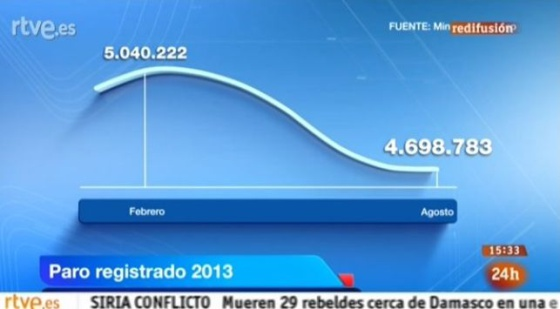
\includegraphics{images/grafico_erroneo1.jpg}
\caption{Fuente: Verne (El País)}
\end{figure}

\begin{figure}
\centering
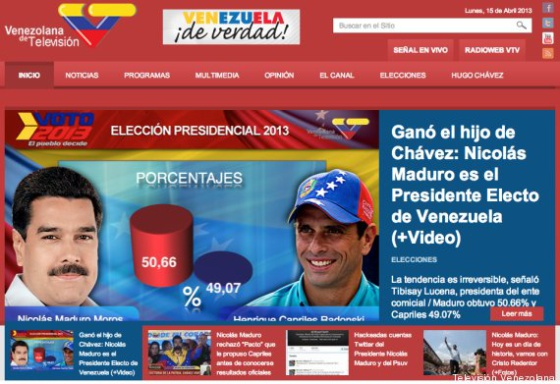
\includegraphics{images/grafico_erroneo2.jpg}
\caption{Fuente: Verne (El País)}
\end{figure}

\begin{figure}
\centering
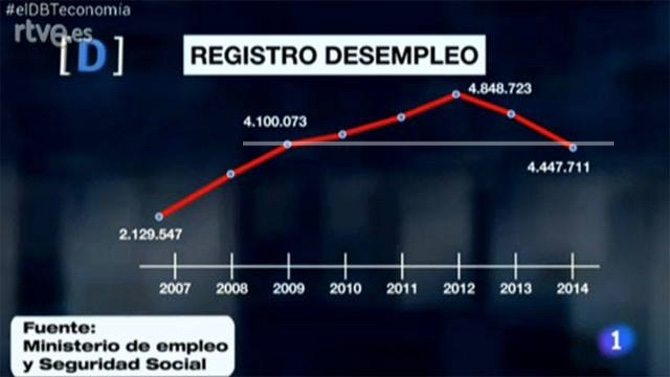
\includegraphics{images/grafico_erroneo3.jpg}
\caption{Fuente: Verne (El País)}
\end{figure}

\begin{enumerate}
\def\labelenumi{\arabic{enumi}.}
\setcounter{enumi}{1}
\tightlist
\item
  No se mantiene la escala en todo el gráfico
\end{enumerate}

\begin{figure}
\centering
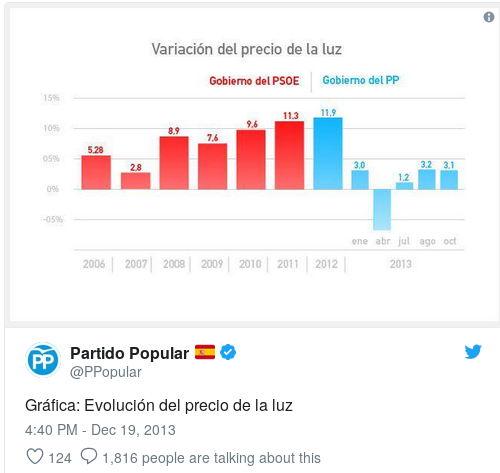
\includegraphics{images/grafico_erroneo4.png}
\caption{Fuente: Verne (El País)}
\end{figure}

\begin{figure}
\centering
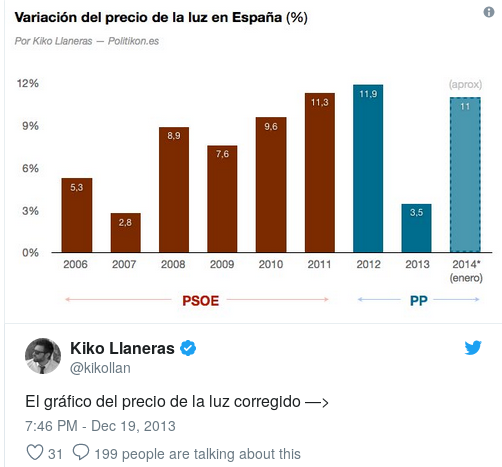
\includegraphics{images/grafico_erroneo4bis.png}
\caption{Fuente: Verne (El País)}
\end{figure}

Se pueden encontrar todos estos gráficos y su expliacción en el diario
\href{https://verne.elpais.com/verne/2015/01/23/articulo/1422014607_223837.html}{El
País} así como en la cuenta de Twitter de
\href{https://twitter.com/kikollan}{Kiko Llaneras}

\section{Medidas de posición central}\label{medidas-de-posicion-central}

\subsection{Medias}\label{medias}

\begin{itemize}
\tightlist
\item
  Una \textbf{media} es una medida de representación central que
  necesariamente debe cumplir tres requisitos:
\end{itemize}

\begin{enumerate}
\def\labelenumi{\arabic{enumi}.}
\tightlist
\item
  Para su obtención deben utilizarse todas las observaciones.
\item
  Debe ser un valor comprendido entre el menor y el mayor de los valores
  de la distribución.
\item
  Debe venir expresada en la misma unidad que los datos.
\end{enumerate}

La media aritmética se calcula mediante la fórmula

\[\overline{x}  =  \frac{\displaystyle\sum_{i=1}^N x_i}{N} = \frac{\displaystyle\sum_{i=1}^r x_i n_i}{N}  =   \sum_{i=1}^r x_i f_i\]

Por ejemplo, la media aritmética de la variable cuantitativa discreta

\[ x_i \]

\[ n_i \]

\[ N_i \]

\[ f_i \]

\[ F_i \]

42

20

20

0.2532

0.2532

43

15

35

0.1899

0.4430

52

20

55

0.2532

0.6962

53

10

65

0.1266

0.8228

62

9

74

0.1139

0.9367

63

5

79

0.0633

1.0000

\[\bar{x} = \frac{\displaystyle\sum_{i=1}^r x_i n_i}{N} = \frac{42\cdot 20 + 43 \cdot 15 + \cdots + 63 \cdot 5}{20+15\cdots+5} = \frac{3928}{79}=49.7215\]

En el caso de \textbf{variables continuas} agrupadas en intervalos
tendremos que obtener primero la \textbf{marca de clase}

\[x_i = \frac{l_{-1}+l_i}{2}\]

\[ ( l_{i-1}, l_i  ] \]

\[n_i\]

\[N_i\]

\[f_i\]

\[F_i\]

\[h_i\]

\[ x_i \]

(0,0.2{]}

45

45

0.5696

0.5696

2.8481

0.10

(0.2,0.3{]}

22

67

0.2785

0.8481

2.7848

0.25

(0.3,0.4{]}

7

74

0.0886

0.9367

0.8861

0.35

(0.4,0.6{]}

5

79

0.0633

1.0000

0.3165

0.50

\[\bar{x}=\frac{ 0.1 \cdot 45 + 0.25 \cdot 22 + \cdots + 0.5 \cdot 5}{45+22\cdots+5} = \frac{14.95}{79}=0.1892\]

Otras medias que suelen utilizarse son:

\begin{itemize}
\item
  \textbf{media geométrica}:
  \[\bar{x}_g  =  \sqrt[N]{x_1^{n_1} x_2^{n_2} \ldots x_r^{n_k}}\]
\item
  \textbf{media armónica}:
  \[\bar{x}_a  = \frac{N}{\displaystyle\sum_{i=1}^k\frac{n_i}{x_i}}\]
\item
  \textbf{media ponderada}: Se asigna a cada valor \(x_i\) un peso
  \(w_i\) que depende de la importancia relativa de cada uno de estos
  valores bajo algún criterio:

  \[\bar{x}_p = \frac{\sum_{i=1}^r n_iw_ix_i}{\sum_{i=1}^r n_iw_i}\]
\end{itemize}

\subsection{Propiedades de la media}\label{propiedades-de-la-media}

\begin{enumerate}
\def\labelenumi{\arabic{enumi}.}
\item
  Se cumple que \(\sum_{i=1}^r (x_i - \bar{x})n_i = 0\)
\item
  Dada una transformación lineal \(Y = aX + b\), se cumple que
  \(\bar{y} = a \bar{x} + b\).
\end{enumerate}

Por ejemplo, si sabemos que la media de temperaturas en grados Celsius
de cierta región es \(\bar{x} = 15^{\circ} \mbox{C}\), ¿qué media en
grados Farenheit tendrá dicha región?

\[\bar{y} = 1.8 \cdot 15 + 32 = 59^{\circ} \mbox{F},\] porque el paso de
una temperatura a otra se hace mediante la transformación
\(Y=1.8 X + 32\)

\begin{enumerate}
\def\labelenumi{\arabic{enumi}.}
\setcounter{enumi}{2}
\tightlist
\item
  La media es el valor \(\phi\) que hace mínima la expresión:
  \[\sum_{i=1}^r (x_i - \phi)^2 n_i\]
\end{enumerate}

\subsection{La mediana}\label{la-mediana}

La \textbf{mediana}, \(M_e\), es un valor que, \textbf{una vez ordenados
los datos}, deja la mitad de las observaciones a la izquierda de él y la
otra mitad a la derecha.

El cálculo de la mediana en el caso de las \textbf{variables discretas}
se realiza:

\begin{enumerate}
\def\labelenumi{\arabic{enumi}.}
\tightlist
\item
  Si \(N\) es impar, entonces \[M_e = x_{({\frac{n+1}{2}})}\]
\item
  Si \(N\) es par, entonces
  \[M_e = \frac{x_{({\frac{n}{2}})}+x_{({\frac{n}{2}+1})}}{2}\]
\end{enumerate}

Por ejemplo, en la siguiente tabla de frecuencias

\[ x_i \]

\[ n_i \]

\[ N_i \]

\[ f_i \]

\[ F_i \]

42

20

20

0.2532

0.2532

43

15

35

0.1899

0.4430

52

20

55

0.2532

0.6962

53

10

65

0.1266

0.8228

62

9

74

0.1139

0.9367

63

5

79

0.0633

1.0000

como \(N\) es impar, entonces la mediana es el valor que ocupa la
posición

\[\frac{79+1}{2} = \frac{80}{2} = 40\]

Mirando en la tabla \(M_e = 52\)

Sin embargo, en la siguiente tabla

\[ x_i \]

\[ n_i \]

\[ N_i \]

\[ f_i \]

\[ F_i \]

42

20

20

0.2564

0.2564

43

15

35

0.1923

0.4487

52

20

55

0.2564

0.7051

53

10

65

0.1282

0.8333

62

9

74

0.1154

0.9487

63

4

78

0.0513

1.0000

como \(N\) es par, entonces la mediana es la media de los valores que
ocupan la posión \(\frac{78}{2} = 39\) y \(\frac{78}{2}+1 = 40\).
Mirando en la tabla

\[M_e = \frac{52+52}{2} = 52\]

La mediana en variables continuas agrupadas en intervalos necesita de
una fórmula. Por ejemplo, en el caso de la tabla de frecuencias:

\[ ( l_{i-1}, l_i  ] \]

\[n_i\]

\[N_i\]

\[f_i\]

\[F_i\]

(0,0.2{]}

45

45

0.5696

0.5696

(0.2,0.3{]}

22

67

0.2785

0.8481

(0.3,0.4{]}

7

74

0.0886

0.9367

(0.4,0.6{]}

5

79

0.0633

1.0000

El primer \(N_i\) que es mayor o igual a
\(\frac{50 \cdot 79}{100} = 39.5\) es \(N_1 = 45\), entonces \(M_e\)
está dentro del intervalo \((0, 0.2]\), por tanto

\[M_e = l_{i-1} + \frac{\frac{50 \cdot N}{100} - N_{i-1}}{N_i - N_{i-1}} \cdot a_i\]
\[M_e = 0 + \frac{\frac{50 \cdot 79}{100} - 0}{45 - 0} \cdot 0.2 = 0.1755\]

\subsection{La moda}\label{la-moda}

\begin{itemize}
\item
  La moda absoluta de una distribución es el valor que más veces se
  repite.
\item
  Además de la moda absoluta, aquellos valores que tengan frecuencia
  mayor a la de los valores adyacentes serán relativas.
\end{itemize}

En la distribución 2, 3, 3, 4, 6, 7, 7, 7, 10

\begin{itemize}
\item
  \(M_o= 7\) es la moda
\item
  \(M_{o_r}=3\) es una moda relativa
\end{itemize}

La moda para variables discretas es sencillo. Miramos la frecuencia
absoluta:

\[ x_i \]

\[ n_i \]

\[ N_i \]

\[ f_i \]

\[ F_i \]

42

20

20

0.2564

0.2564

43

15

35

0.1923

0.4487

52

20

55

0.2564

0.7051

53

10

65

0.1282

0.8333

62

9

74

0.1154

0.9487

63

4

78

0.0513

1.0000

En este caso, el valor que más se repite es \(M_o = 42\)

En el caso de variables continuas tendremos que utilizar una fórmula:

\[ ( l_{i-1}, l_i  ] \]

\[n_i\]

\[N_i\]

\[f_i\]

\[F_i\]

\[h_i\]

\[ x_i \]

(0,0.2{]}

45

45

0.5696

0.5696

2.8481

0.10

(0.2,0.3{]}

22

67

0.2785

0.8481

2.7848

0.25

(0.3,0.4{]}

7

74

0.0886

0.9367

0.8861

0.35

(0.4,0.6{]}

5

79

0.0633

1.0000

0.3165

0.50

En lugar de fijarnos en \(n_i\) nos fijamos en \(h_i\). Como el mayor
\(h_i\) es 2.8481 la moda es

\[M_o = l_{i-1} + \frac{ h_{i+1} }{ h_{i-1}+h_{i+1} } \cdot a_i\]

\[M_o = 0 + \frac{2.7848}{0+2.7848} \cdot 0.2 = 0.2\]

\section{Medidas de dispersión}\label{medidas-de-dispersion}

\subsection{Varianza y Desviación
Típica}\label{varianza-y-desviacion-tipica}

\begin{itemize}
\tightlist
\item
  La \textbf{varianza}, \(S^2\), y su raíz cuadrada positiva, la
  \textbf{desviación típica}, \(S\), son las medidas de dispersión más
  importantes.
\end{itemize}

\(S^2 = \frac{\sum_{i=1}^r ( x_i - \bar{x})^2 n_i}{N} = \frac{\sum_{i=1}^r x_i^2 n_i}{N} - \bar{x}^2 \qquad S=+\sqrt{S^2}\)

\begin{enumerate}
\def\labelenumi{\arabic{enumi}.}
\item
  La desviación típica viene dada en las mismas unidades que la variable
  estadística.
\item
  Tanto \(S\) como \(S^2\) son siempre no negativas y valen cero sólo en
  el caso de que todos los valores coincidan con la media.
\item
  Los valores atípicos influyen en las dos debido al cálculo de la
  media.
\end{enumerate}

\subsection{Propiedades de la
varianza}\label{propiedades-de-la-varianza}

\begin{itemize}
\tightlist
\item
  Si \(Y=aX + b\) entonces se verifica \(S_Y^2 = a^2 S_X^2\). Por
  ejemplo
\end{itemize}

Dada \(X\) con \(\bar{x}=12\) y \(S_X=9\), entonces para \(Y=3X-4\):

\[\bar{y}=3\bar{x}-4=3\cdot 12-4=32\]
\[S_Y=\sqrt{a ^2}\cdot S_X=\sqrt{9}\cdot 9=27\]

\subsection{Coeficiente de Variación}\label{coeficiente-de-variacion}

\[C_v = \frac{S}{\mid \bar{x}\mid}\]

\begin{enumerate}
\def\labelenumi{\arabic{enumi}.}
\item
  Permite comparar la dispersión de varias distribuciones.
\item
  Da información sobre la representatividad de la media. De forma
  orientativa, si el coeficiente de variación es menor o igual a 0.5
  diremos que la media es representativa.
\end{enumerate}

\subsection{Otras medidas de
dispersión}\label{otras-medidas-de-dispersion}

\begin{itemize}
\item
  El \textbf{rango} es la diferencia entre el mayor y el menor de los
  valores de la variable.
\item
  La \textbf{desviación media}
  \[D_m = \frac{\sum_{i=1}^r |  x_i - \bar{x} | n_i}{n}\]
\end{itemize}

\subsection{Desigualdad de Tchebychev (para
ampliar)}\label{desigualdad-de-tchebychev-para-ampliar}

La desigualdad de Tchebychev proporciona una cota inferior para el
porcentaje de observaciones en un determinado intervalo con centro la
media de la distribución:

Dada una distribución con \(\bar{x}=25\), y \(S=4\),
\([\bar{x}-3S,\bar{x}+3S]=[13,37]\) garantiza la presencia en su
interior de, al menos, el \(88.88\%\) de la distribución.

\section{Medidas de posición no
central}\label{medidas-de-posicion-no-central}

Se llaman medidas de posición o de orden \(k\) a aquellas que dividen a
la distribución en \(k\) partes, de tal forma que en cada una de esas
partes haya el mismo número de elementos. Las más importantes son:

\begin{itemize}
\item
  Los \textbf{cuartiles}, \(Q_i, i=1,2,3\) que dividen a la distribución
  en cuatro partes iguales.
\item
  Los \textbf{deciles} , \(D_i, i=1,2, \ldots, 9\) que dividen a la
  distribución en diez partes iguales.
\item
  Los \textbf{percentiles}, \(P_i, i=1,2, \ldots, 99\) que dividen a la
  distribución en cien partes iguales.
\end{itemize}

El cálculo de los percentiles será suficiente para calcular tanto los
deciles como los cuartiles. En el caso de variables discretas:

\begin{itemize}
\tightlist
\item
  Si el \(k\%\) de \(N\), donde \(N\) es el número de datos, es un
  número entero, \(r\), entonces
\end{itemize}

\[P_k = \cfrac{x_r+x_{r+1}}{2}\]

\begin{itemize}
\tightlist
\item
  Si el \(k\%\) de \(N\) no es un número entero, lo redondeamos al
  siguiente, \(r\), u entonces
\end{itemize}

\[P_k = x_r\]

Para el caso de datos agrupados en intervalos utilizaremos la fórmula:

\[P_k = l_{i-1} + \cfrac{\cfrac{k \cdot N}{100} - N_{i-1}}{N_i -N_{i-1}} \cdot a_i\]
donde \(N_i\) es la primera frecuencia absoluta acumulada que cumple
\(N_i \geq \cfrac{k \cdot N}{100}\)

\subsection{Diagrama de caja}\label{diagrama-de-caja}

Es una representación gráfica de los cuartiles:

\begin{itemize}
\item
  La caja representa el 50\% central de la distribución, la línea
  situada en el interior de la caja es la mediana (algunos programas
  estadísticos representan también un símbolo que se corresponde con la
  media).
\item
  La longitud de la caja es el \textbf{rango intercuartílico}
  \(R_I = Q_3 - Q_1\)
\item
  Los extremos inferiores y superiores de los segmentos encierran los
  valores ``normales''.
\item
  Los candidatos a valores anómalos se etiquetan como \textbf{atípicos}
  y se encuentran fuera del intervalo
  \((Q_1 - 1.5 \cdot R_I,Q_3 + 1.5 \cdot R_I)\):
\end{itemize}

\[ ( l_{i-1}, l_i  ] \]

\[n_i\]

\[N_i\]

(0,0.2{]}

45

45

(0.2,0.3{]}

22

67

(0.3,0.4{]}

7

74

(0.4,0.6{]}

5

79

Los percentiles 25, 50 y 75 de la concentración de fluoruro son 0.13,
0.18, 0.28 respectivamente. Además \(1.5 \cdot R_I\) es 0.225

\begin{center}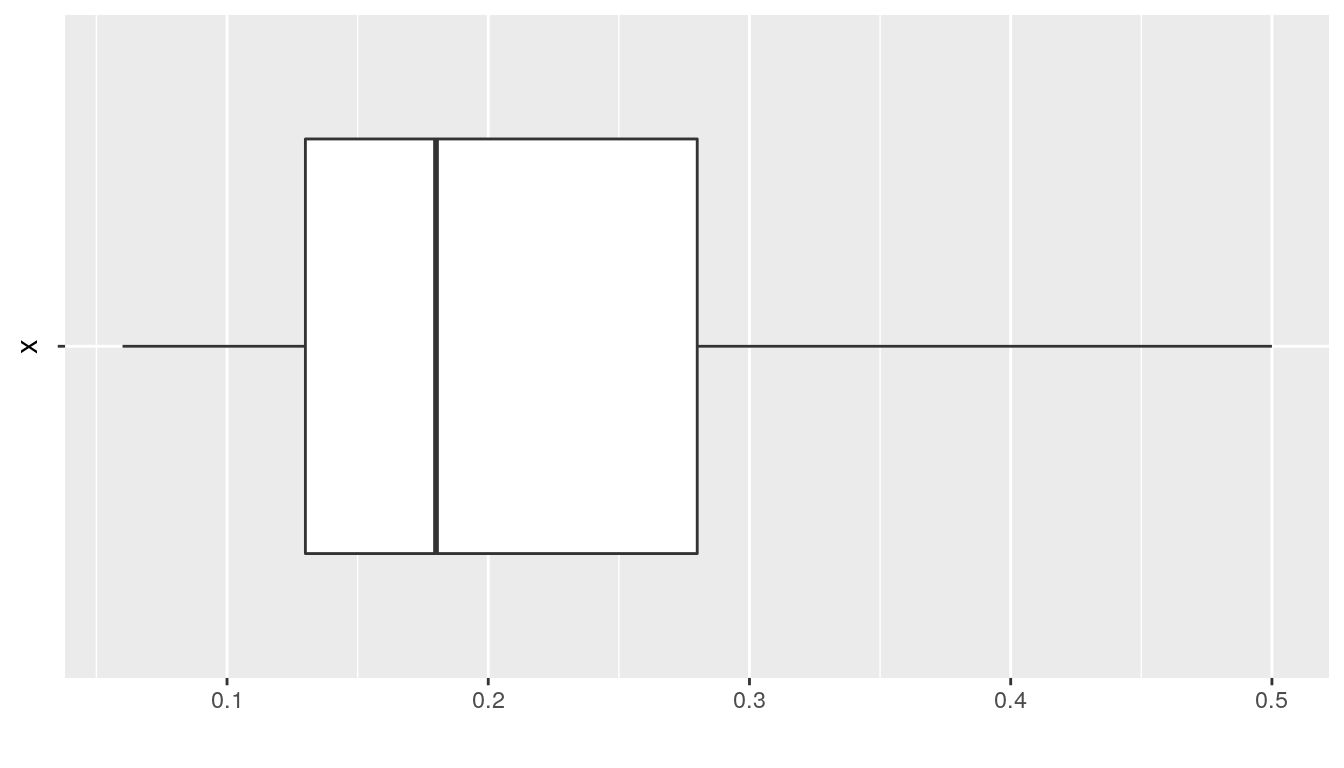
\includegraphics{01-AnalDatos_files/figure-latex/unnamed-chunk-21-1} \end{center}

\section{Medidas de forma}\label{medidas-de-forma}

\subsection{Asimetría}\label{asimetria}

\begin{itemize}
\tightlist
\item
  El \textbf{coeficiente de simetría} viene dado por:
  \[\gamma_1 = \frac{\sum_{i=1}^N (x_i - \bar{x})^3}{N \cdot S^3}\]
\end{itemize}

Observe que cuando la distribución es simétrica coinciden la media y la
mediana. Si la distribución tiene además forma de campana, la media y la
mediana se aproximan a la moda.

\begin{center}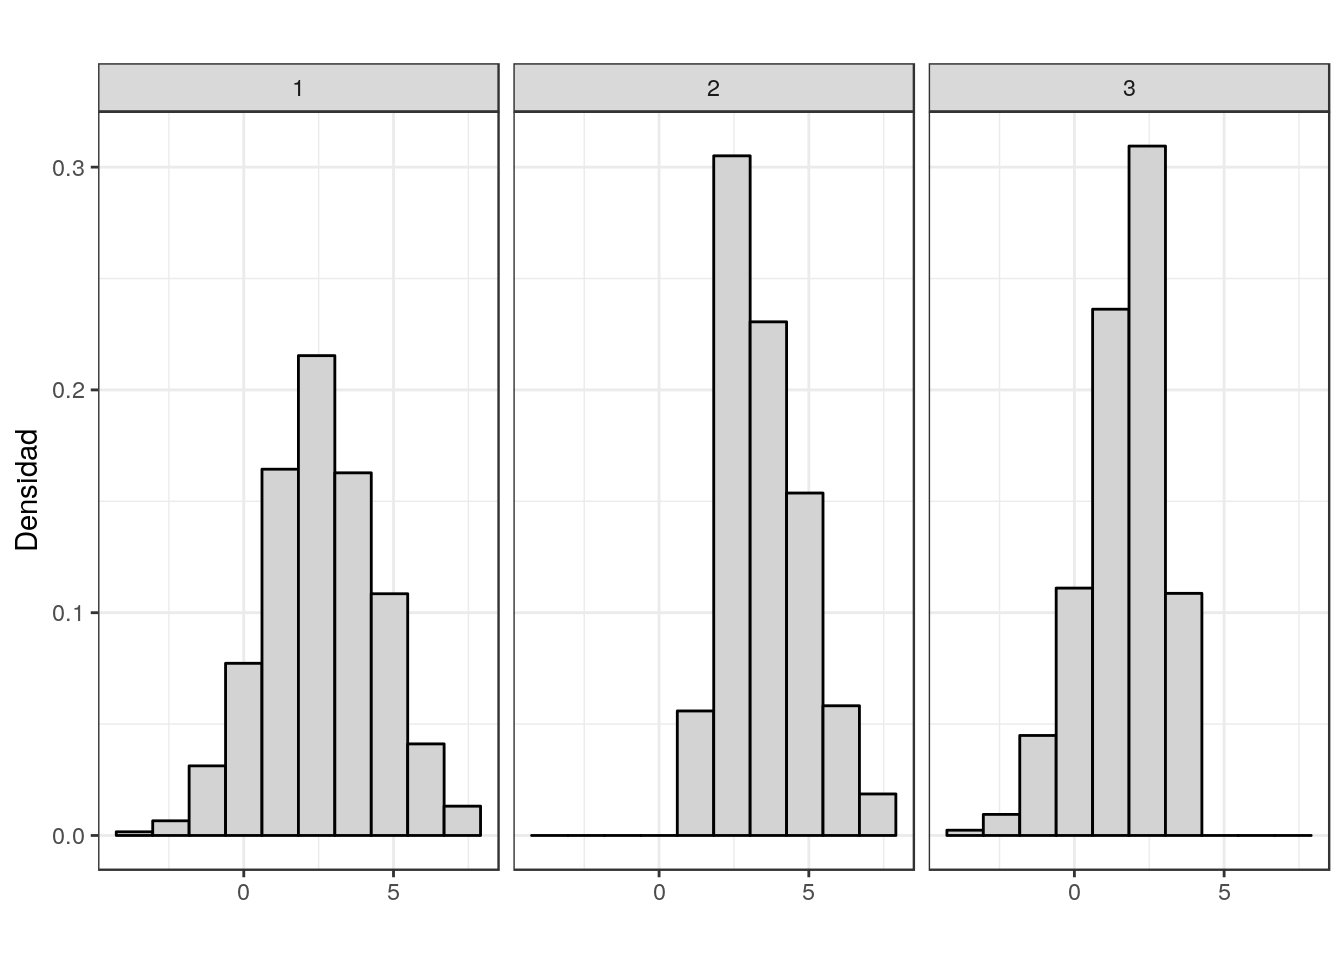
\includegraphics{01-AnalDatos_files/figure-latex/unnamed-chunk-22-1} \end{center}

En estos casos, la asimetría es, de izquierda a derecha, 0.0491772,
0.776285, -0.6764108, respectivamente.

\subsection{Curtosis}\label{curtosis}

Para el cálculo de la curtosis utilizaremos
\[\gamma_2  =  \frac{\sum_{i=1}^N (x_i - \bar{x})^4}{N \cdot S^4}-3\]

\begin{itemize}
\item
  \(\gamma_2= 0\), distribución \textbf{mesocúrtica}
\item
  \(\gamma_2< 0\), distribución \textbf{platicúrtica}
\item
  \(\gamma_2> 0\), distribución \textbf{leptocúrtica}
\end{itemize}

\begin{center}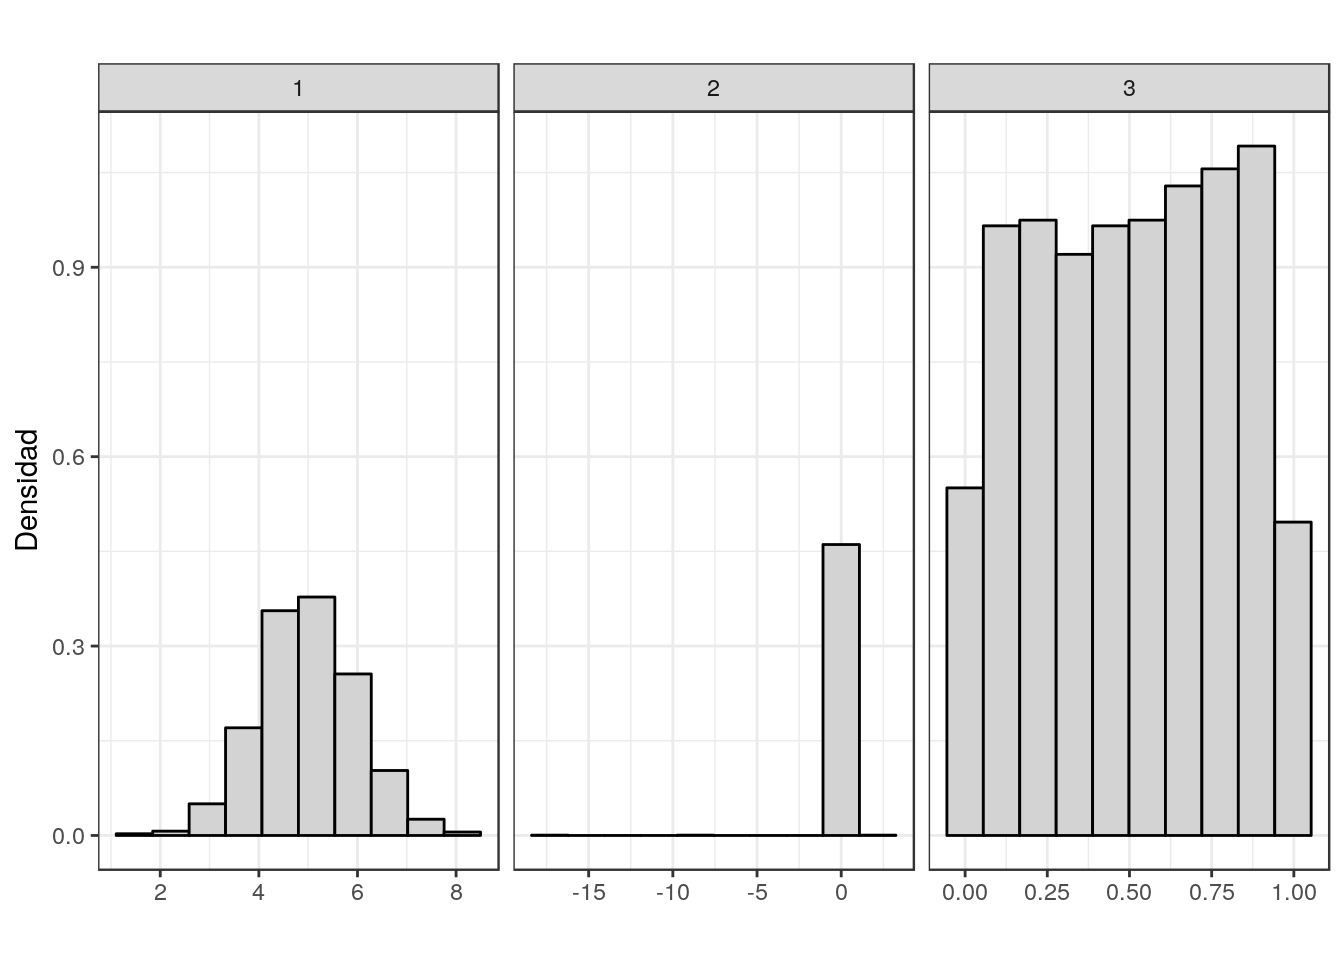
\includegraphics{01-AnalDatos_files/figure-latex/unnamed-chunk-23-1} \end{center}

En las distribuciones anteriores, y de izquierda a derecha, las curtosis
tienen un valor de

-0.2832262, 385.208987, 0.0683932, respectivamente.

Puede verse una aplicación de cómo el histograma y el diagrama de caja
tienen un comportamiento similar ante diferentes formas de la
distribución en la siguiente aplicación:

\begin{Shaded}
\begin{Highlighting}[]
\NormalTok{knitr}\OperatorTok{::}\KeywordTok{include_app}\NormalTok{(}\StringTok{"https://berihuete.shinyapps.io/Histogram/"}\NormalTok{, }
  \DataTypeTok{height =} \StringTok{"600px"}\NormalTok{)}
\end{Highlighting}
\end{Shaded}

\section{Tipificación}\label{tipificacion}

A veces la distribución presenta muchas irregularidades, como asimetrías
acentuadas, valores extremos, etc. En estos casos es recomendable
efectuar una transformación que la haga más regular. Un caso particular
de transformación es la \textbf{tipificación}.

Dada \(X\) con media \(\bar{x}\) y desviación típica \(S\)

\[Z  =  \frac{X  -  \bar{x}}{S}\]

A \(Z\) se le llama variable o y tiene media 0 y desviación típica 1.

La tipificación tiene la propiedad de hacer comparables individuos que
pertenezcan a distintas distribuciones, aún en el caso de que éstas
vinieran expresadas en diferentes unidades.

Dos trabajadores del mismo sector ganan 620 y 672 euros,
respectivamente. El primero pertenece a la empresa A, cuya retribución
media y desviación típica vienen dados por: \(\bar{x}_A= 580\) euros y
\(S_{x_A} = 25\) euros, mientras que para la empresa del segundo
trabajador se tiene: \(\bar{x}_B\) =640 euros y \(S_{x_B} = 33\) euros.

¿cuál de los dos ocupa mejor posición relativa dentro de su empresa?
\[z_A=\frac{620-580}{25}=1.6\]

\[z_B=\frac{672-640}{33}=0.97\]

\chapter{Análisis bivariante. Ajuste y regresión
bidimensional.}\label{analisis-bivariante.-ajuste-y-regresion-bidimensional.}

\chapter{Objetivos del tema:}\label{objetivos-del-tema}

Cuando analizamos dos variables estadísticas a la vez, hablamos de
\textbf{estadística descriptiva bivariante}. Si hay más de dos, hablamos
de \textbf{estadística descriptiva multivariante}. Por ejemplo:

\begin{longtable}[]{@{}cc@{}}
\toprule
X & Y\tabularnewline
\midrule
\endhead
14 & 3\tabularnewline
12 & 4\tabularnewline
15 & 1\tabularnewline
13 & 5\tabularnewline
16 & 0\tabularnewline
\bottomrule
\end{longtable}

Una observación de esta variable bidimensional es \((14,3)\).

Los objetivos que nos planteamos para este capítulo son:

\begin{itemize}
\item
  Organizar los datos en tablas de frecuencias, buscando la mejor forma
  de representarlos gráficamente.
\item
  Medir la relación entre dos variables estadísticas cualitativas.
\item
  Medir la relación entre dos variables estadísticas cuantitativas.
\item
  Realizar predicciones y medir la fiabilidad de dicha predicción.
\item
  Entender que \textbf{la correlación no implica causalidad}.
\end{itemize}

\bibliography{book.bib,packages.bib}


\end{document}
